\documentclass[12pt]{article}
\usepackage{makeidx}
\makeindex
\usepackage{subcaption}
\usepackage[utf8]{inputenc}%acentuação das palavras
\usepackage[T1]{fontenc}%codificação de fonte
\usepackage[brazilian]{babel}
\usepackage{tikz}
\usepackage{textcomp}
\usepackage{afterpage}
\usepackage{varwidth}
\usepackage{indentfirst}
\usepackage{amsfonts}
\usepackage{amsmath}
\usepackage{amsthm}
%\usepackage{amssymb}
\usepackage{amscd}
\usepackage{amsxtra}
\usepackage{latexsym}
\usepackage{hyperref}
%\usepackage{cleveref}
\usepackage{enumerate}
\usepackage{fancyhdr}
\usepackage{etoolbox}
\usepackage{multicol}
\usepackage{multirow}
\usepackage{setspace} \onehalfspacing
\usepackage{mathptmx}
\usepackage[portuguese,ruled,vlined,linesnumbered]{algorithm2e}%algoritmos
\setlength{\parindent}{1.5cm}
\usepackage[a4paper,top=3cm,bottom=2cm,left=3cm,right=2cm,marginparwidth=1.75cm]{geometry}
\usepackage{lastpage}
\usepackage{fancyhdr}

\usepackage[italic]{mathastext}
\usepackage{graphicx}
\usepackage{longtable}

\title{Projeto 4 - MS960/MT862}
\author{Fernando Ribeiro de Senna --- RA 197019\\
Rodolfo da Silva Santos --- RA 228711}
\date{08 de janeiro de 2021}
\begin{document}
\maketitle

A Seção \ref{parte1} versa sobre a implementação computacional da parte 1 do projeto e a Seção \ref{parte2} apresenta o que foi feito na parte 2 do projeto.

Foram utilizados funções e objetos das bibliotecas \textit{pandas, numpy, scipy} e \textit{matplotlib}. 

Toda a fundamentação teórica se baseia em conteúdo oferecido em vídeo-aulas e \textit{slides} pelo Professor João Batista Florindo em ocasião de oferecimento da disciplina MS960 no segundo semestre de 2020 pelo Instituto de Matemática, Estatística e Computação Científica (IMECC) da Universidade Estadual de Campinas (UNICAMP).




\section{Detecção de Anomalias ---Parte I} \label{parte1}

Essa seção explica a implementação de modelos de detecção de anomalias em servidores computacionais usando o modelo Gaussiano multivariado.

Para isso foi utilizado os dados presentes nos arquivos dados1.mat e que contém um conjunto de exemplos de servidores (matriz X), cada um com sua respectiva latência (tempo que um pacote específico leva para chegar ao destino) na $1^{a}$ coluna e taxa de transferência (quantidade de dados transferidos de um lugar para outro) na $2^{a}$ coluna. Estes arquivos também possuem uma matriz Xval com um conjunto de dados de validação e um vetor yval com seus respectivos rótulos.

O arquivo dados2.mat armazena matrizes com 11 parâmetros relacionados ao funcionamento dos servidores e possuem uma quantidade maior de exemplos de treinamento. Ele será utilizado em testes complementares com o sistema desenvolvido.

A implementação descrita na presente Seção foi feita em linguagem python em arquivo do tipo notebook e pode ser encontrada no arquivo Anomaly\_Proj4\_Par1.ipynb. Inicialmente, importam-se as bibliotecas numpy e matplotlib, loadmat da biblioteca scipy.io e o módulo seaborn do python. Os detalhes da implementação estão descritos nas próximas seções.

\subsection{Ajuste da Gaussiana multivariada aos dados} \label{gau_mult}
Para realizar a detecção de anomalias foi desenvolvido um modelo de distribuição dos dados. O conjunto de treinamento $x^{(1)},…, x^{(m)}$, com $x^{(i)} \in R ^ n$, foi utilizado para gerar uma estimativa da distribuição gaussiana para cada um dos exemplos de treinamento. Para cada um deles (i = 1 ... n), foi encontrada  a média $\mu$ e a variância $\sigma^{2}$. As funções que calculam a média e a variância estão abaixo. No código foram implementadas na função estimateGaussian( ) que recebe uma matriz X com os exemplos de treinamento e retorna a média $\mu$ e a variância $\sigma^{2}$.

\begin{equation} \label{eq_mu}
\mu_{j} = \frac{1}{m}\sum^{m}_{i=1}x^{(i)}_{j} 
\end{equation}

\begin{equation} \label{eq_sig}
\sigma^{2}_{j} = \frac{1}{m}\sum^{m}_{i=1}(x^{(i)}_{j} - \mu_{j})^{2} 
\end{equation}

Ao calcular a média para cada exemplo, calculamos a variância dos exemplos correspondentes. 

Uma vez que encontradas a média e a variância precisamos calcular a probabilidade dos exemplos de treinamento para decidir quais exemplos são anômalos. 
A distribuição gaussiana multivariada foi usada para encontrar a probabilidade de cada exemplo de treinamento e com base em algum valor limite - valor de $\epsilon$ - sinaliza se é uma anomalia ou não. A expressão para calcular as probabilidades com modelo de distribuição Gaussiana multivariada é:

\begin{equation} \label{eq_p}
p(x) = (x;\mu;\Sigma) = \frac{1}{(2\pi)^{n/2}|\Sigma|^{1/2}}exp(-\frac{1}{2}(x-\mu)^{T}\Sigma^{-1}(x - \mu)) 
\end{equation}

Em que $\Sigma$ é a matriz de covariância e $|\Sigma|$ o determinante de $\Sigma$. No código está função foi implementada em multivariateGaussian( ) e recebe como valore de entrada uma matriz X com os exemplos de treinamento e os valores de $\mu$ e $\sigma^2$, retornando o vetor p com os valores das probabilidades calculadas para cada exemplo de treinamento.

Temos uma anomalia se p(x) < $\epsilon$.


\subsection{Curvas de contorno da Gaussiana} \label{cur_gau}
No ajuste das curvas de contorno da gaussiana foi utilizada a função kdeplot do módulo python seaborn. O kdeplot cria gráficos de estimativa de distribuição de kernel que representa a função de densidade de probabilidade das variáveis de dados contínuas ou não paramétricas, ou seja, pode-se representar graficamente as variáveis univariadas ou múltiplas ao mesmo tempo. O kdeplot utiliza um algoritmo de kernel gaussiano para gerar as curvas de probabilidades.

A função kdeplot recebe a matriz de dados e um parâmetro de suavização das curvas bw. Após o ajuste manual do parâmetro bw foi obtido o seguinte gráfico.

\begin{figure} [htp]
\begin{center}
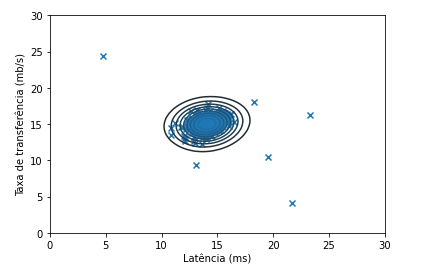
\includegraphics[scale=0.8]{curvas.png}
\caption{Curvas de contorno da
Gaussiana obtida} \label{curvas}
\end{center}
\end{figure}

Com essas curvas de contorno da gaussiana podemos identificar facilmente os pontos que fogem do padrão esperado.

\subsection{Valor ideal de $\epsilon$ e $F_{1}-score$} \label{}

Encontradas as probabilidades para os dados (no código estas probabilidades foram armazenadas na variável pval), em seguida é necessário determinar os valores ótimos do threshold $\epsilon$ e do $F_{1}-score$ utilizando dados rotulados. Esses parâmetros são calculados na função selectThreshold( ) que recebe os vetores pval com as probabilidades de cada exemplo de treinamento e o vetor yval com os rótulos de cada exemplo de treinamento. 

Antes de se calcular esses parâmetros o pval foi dividido em subintervalos entre o máximo e o mínimo possível de threshold. Permitindo, assim, a verificação de um determinado número de $\epsilon$ entre o maior e o menor $\epsilon$ presente em pval. No projeto foram utilizados 1000 intervalos. Para cada valor de $\epsilon$ no vetor epi\_range se calcula a predição. Ou seja, se os valores presentes no vetor pval forem menores que o $\epsilon$ da interação, a predição retornará 1 (positivo para anomalia), caso contrário receberão 0 (negativo para anomalia). Na função selectThreshold( ) isso é feito criando-se o vetor predictions que conterá a comparação entre o vetor pval e o $\epsilon$ da interação. Em seguida, se calcula o número de verdadeiro-positivos, falso-positivos e falso-negativos comparando-se os vetores predictions e yval. 

O precision e o recall são calculados respectivamente pelas fórmulas tp/(tp+fp) e tp/(tp+fn). Por fim, a cada interação, o $F_{1}-score$ é calculado pela fórmula (2*prec*rec)/(prec+rec) e comparado com o $F_{1}-score$ da interação anterior. Se o $F_{1}-score$ for maior que o da interação anterior, o $\epsilon$ e $F_{1}-score$ são atualizados pelos valores recém calculados. No fim do processo os valores de $\epsilon$ e $F_{1}-score$ são retornados pela função.

\subsection{Localizando e circulando as Anomalias} \label{lc_ano}

Em posse do melhor valor para $\epsilon$ podemos encontrar as anomalias/ outliers por meio da probabilidade dos exemplos de treinamento. Os outliers serão aqueles que possuem probabilidades menores que o $\epsilon$ ótimo. 
outliers = p < $\epsilon$

Através da comparação do vetor pval com o valor do $\epsilon$ ótimos os índices dos outliers são armazenados no vetor outliers permitindo sua posterior identificação no gráfico. A imagem a seguir mostra o gráfico com as anomalias circuladas em vermelho.

\begin{figure} [htp]
\begin{center}
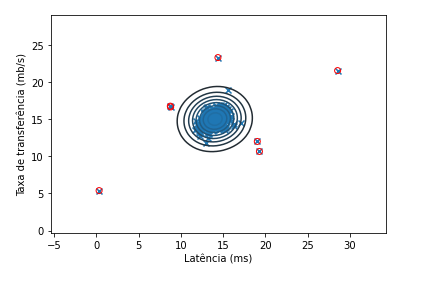
\includegraphics[scale=0.8]{anomalias.png}
\caption{Anomalias circuladas em vermelho} \label{anomalias}
\end{center}
\end{figure}

Como pode ser visto no gráfico, 7 anomalias  foram detectadas pelo modelo (os pontos 8.73/16.79 e 8.77/16.68 ficaram sobrepostos). Nesse modelo de detecção de anomalias os valores de $\epsilon$ e $F_{1}-score$ foram 8.990852779269495e-05 e 0.8750000000000001 respectivamente. E pela análise visual desses pontos se verifica que eles são exatamente os pontos que fogem do padrão esperado. 

\subsection{Outro exemplo de detecção de Anomalias} \label{}

Ao executar o sistema desenvolvido com os dados do arquivo dados2.mat obteve-se valores para $\epsilon$ e $F_{1}-score$ iguais a 1.3772288907613575e-18 e 0.6153846153846154 respectivamente. Como os exemplos de treinamento possuem muitos parâmetros não é possível uma inspeção visual das anomalias encontradas. 

Dezesseis anomalias foram encontradas e seus respectivos índices são: [0, 3, 6, 11, 19, 27, 34, 43, 50, 59, 60, 69, 71, 86, 88, 92].


\section{Sistema de Recomendação --- Parte II} \label{parte2}

Essa Seção explica a implementação realizada para construção de um sistema de recomendação de filmes. A Seção \ref{doc_rec} apresenta a documentação das funções implementadas no arquivo \textit{functions\_recomendacao.py}. Já a Seção \ref{treino_rec} apresenta a importação dos dados e o treinamento do algoritmo e a Seção \ref{notas_rec} apresenta os resultados e as notas obtidos, implementados no arquivo \textit{Parte2\_Recomendacao.ipynb}.

O problema se baseia em partir de notas atribuídas a filmes por usuários e, com isso, treinar um algoritmo que seja capaz de "prever" \ as notas que os usuários dariam aos filmes que eles não viram e fazer recomendações.

Os dados iniciais do problema são representados por matrizes $Y, R \in \Re^{m \times n}$. Cada entrada (i,j) da matriz Y corresponde à nota (de 1 a 5) dada pelo usuário j ao filme i, enquanto as entradas (i,j) da matriz R valem 1 se o usuário j atribuiu alguma nota ao filme i e 0 caso contrário. Quando não houve atribuição de nota a um filme por um usuário, a entrada correspondente da matriz Y é nula.

A partir disso, desejamos construir uma matriz X, em que cada linha representa um vetor $x^{(i)}$ de atributos relativos ao filme i, e uma matriz $\Theta$, em que cada linha representa vetor $\theta^{(j)}$ de parâmetros do usuário j. Uma vez em posse dessas matrizes, é possível obter matriz $X\Theta^t$, cuja entrada (i,j) representa a nota prevista para o usuário j dar ao filme i, como em uma regressão linear. A obtenção das matrizes X e $\Theta$ é feita através de treinamento do algoritmo de recomendação com minimização através de algoritmo de gradiente conjugado.

\subsection{Documentação} \label{doc_rec}
Essa Seção apresenta as funções utilizadas para criação do sistema de recomendação, implementadas no arquivo \textit{functions\_recomendacao.py.}

\subsubsection{Função \textit{cost\_fun}}
Função que calcula o valor da função de custo do problema e seu gradiente com relação às variáveis x e $\theta$.

Argumentos de entrada:

\begin{description}
\item[variables] Vetor que corresponde à concatenação das matrizes X e $\Theta$, após serem convertidas em vetores.
\item[Y] Matriz em que a entrada (i,j) representa a nota dada pelo usuário j ao filme i.
\item[R] Matriz em que a entrada (i,j) vale 1 se o usuário j deu nota ao filme i e 0, caso contrário.
\item[n\_pars] Dimensão dos vetores de atributos e parâmetros $x^{(i)}$ e $\theta^{(j)}$.
\end{description}

A função retorna:

\begin{description}
\item[J] Valor da função de custo
\item[grad] Vetor que representa o gradiente da função de custo com relação aos atributos e parâmetros $x^{(i)}$ e $\theta^{(j)}$.
\end{description}

Inicialmente, a função reconstrói as matrizes X e $\Theta$ a partir do vetor \textit{variables}. Em seguida, calcula o valor da função de custo J através da Equação \ref{eq_J} e as matrizes  que representam o gradiente de J com relação a cada entrada de X e de $\Theta$ através das Equações \ref{eq_grad_x} e \ref{eq_grad_theta}. Por fim, essas matrizes são convertidas em vetor em concatenadas para gerar o vetor \textit{grad}. 

\begin{equation} \label{eq_J}
J = \frac{1}{2} \sum_{i,j: R(i,j) = 1} \left[\left(\theta^{(j)}\right)^t x^i - y^{(i,j)}\right]^2 
\end{equation}

\begin{equation} \label{eq_grad_x}
\nabla_X^{(i,k)} = \sum_{j:R(i,j)=1} \left[\left(\theta^{(j)}\right)^t x^i - y^{(i,j)}\right]\theta^{(j,k)}
\end{equation}

\begin{equation} \label{eq_grad_theta}
\nabla_{\Theta}^{(j,k)} = \sum_{i:R(i,j)=1} \left[\left(\theta^{(j)}\right)^t x^i - y^{(i,j)}\right]x^{(i,k)}
\end{equation}

\subsubsection{Função \textit{normalizacao}}
Função que realiza normalização de matriz Y de notas fornecidas por usuários.

Argumentos de entrada:

\begin{description}
\item[Y] Matriz em que a entrada (i,j) representa a nota dada pelo usuário j ao filme i.
\item[R] Matriz em que a entrada (i,j) vale 1 se o usuário j deu nota ao filme i e 0, caso contrário.
\end{description}

A função retorna:

\begin{description}
\item[norm] Matriz Y normalizada
\item[media] Vetor com as médias das notas dadas para cada filme
\end{description}

Essa função calcula a média de notas dadas para cada um dos filmes (desconsiderando, no cálculo, os usuários que não deram nota para o filme), obtendo vetor de notas médias. Em seguida, realiza-se subtração da média de cada uma das notas dadas, obtendo a matriz de notas normalizadas. Note que as entradas de \textit{norm} correspondentes às entradas nulas de Y continuam nulas.

Em normalizações, é comum fazer a subtração da média e, em seguida, dividir pelo desvio padrão. Contudo, isso não foi feito, pois em alguns casos, há poucos usuários que deram notas ao filme, tornando o desvio padrão pouco representativo.

\subsubsection{Função \textit{treinamento}}
Função que realiza treinamento do algoritmo.

Argumentos de entrada:

\begin{description}
\item[Y] Matriz em que a entrada (i,j) representa a nota dada pelo usuário j ao filme i.
\item[R] Matriz em que a entrada (i,j) vale 1 se o usuário j deu nota ao filme i e 0, caso contrário.
\item[n\_pars] Dimensão dos vetores de atributos e parâmetros $x^{(i)}$ e $\theta^{(j)}$.
\item[n\_iter] Número máximo de iterações com o algoritmo de gradiente conjugado que podem ser realizadas. 
\end{description}

A função retorna:

\begin{description}
\item[X] Matriz  em que cada linha representa um vetor $x^{(i)}$ de atributos relativos ao filme i.
\item[$\Theta$] Matriz em que cada linha representa vetor $\theta^{(j)}$ de parâmetros do usuário j
\item[res] Objeto da biblioteca \textit{scipy.optimize} que apresenta detalhes da otimização realizada.
\end{description}

A função constrói matrizes $X \in \Re^{m \times n\_pars}$ e $\Theta \in \Re^{n \times n\_pars}$ de entradas aleatoriamente geradas pela função \textit{rand} da biblioteca \textit{numpy.random.} Em seguida, ela transforma essas matrizes em vetores e os concatena, passando esses valores como valores iniciais da função \textit{minimize} da biblioteca \textit{scipy.optimize} que realiza minimização irrestrita da função de custo J através de algoritmo de gradiente conjugado aplicado sobre a função \textit{cost\_fun}. Por fim, a função reconstrói as matrizes X e $\Theta$ obtidas após a otimização.

\subsection{Importação dos dados e treinamento} \label{treino_rec}
A implementação descrita na presente Seção foi feita em linguagem \textit{python} e arquivo tipo \textit{notebook} e pode ser encontrada no arquivo \textit{Parte2\_Recomendacao.ipynb.}

Inicialmente, importam-se as bibliotecas \textit{numpy e pandas}, além da função \textit{loadmat} da biblioteca \textit{scipy.io} e das funções do arquivo \textit{functions\_recomendacao.ipynb}, descritas na Seção \ref{doc_rec}.

Em seguida, os dados do problema são importados. As matrizes Y e R, conforme descritas anteriormente, são importadas do arquivo \textit{dado3.mat} e a lista de filmes do arquivo \textit{dado4.txt.}

Antes de realizar o treinamento, uma rotina percorre todas as linhas e colunas da matriz R e informa se todos os filmes receberam ao menos uma nota e todos os usuários deram ao menos uma nota. Isso é importante, pois, caso algum filme não receba nenhuma classificação ou algum usuário não forneça nenhuma nota, é necessário alterar a matriz Y, de forma que a esse filme/usuário seja atribuído comportamento médio com relação aos demais, a fim de garantir que o algoritmo implementado tenha um bom desempenho. Como na base de dados utilizados todos os usuários deram ao menos uma nota e todos os filmes receberam ao menos uma nota, não é necessário fazer nenhuma modificação.

Uma vez feita essa verificação, realiza-se normalização da matriz Y através da função \textit{normalizacao}. Define-se a variável \textit{n\_pars} como o tamanho dos vetores $x^{(i)}$ e $\theta^{(j)}$ (foi utilizado valor 100) e a variável $n\_iter$ que indica o número máximo de iterações permitido (n\_iter=10000). Por fim, o algoritmo é treinado através da função \textit{treinamento.}

O algoritmo de otimização obteve sucesso após 8943 iterações, sem ser necessário atingir o limite de 10000 iterações previamente definido. O valor da função de custo obtido ao fim da otimização é cerca de $2,55 * 10^{-7}$.

\subsection{Previsão das notas} \label{notas_rec}
A implementação descrita na presente Seção foi feita em linguagem \textit{python} e arquivo tipo \textit{notebook} e pode ser encontrada no arquivo \textit{Parte2\_Recomendacao.ipynb.} É uma continuação do que foi feito na Seção \ref{treino_rec}.

Uma vez finalizado o treinamento, calculam-se as notas previstas através da multiplicação de matrizes $X\Theta^t$ e elas são comparadas com as notas fornecidas pelos usuários nos exemplos de treinamento. Com precisão $\epsilon = 10^{-2}$, a diferença entre todas as notas previstas e as notas dadas pelos usuários é nula, assim como o valor da função objetivo.

Com base nos resultados obtidos, combinam-se as notas previamente fornecidas pelos usuários com as notas previstas pelo sistema de recomendação (para os pares de filmes/usuários em que não existe atribuição de nota) e calculam-se as notas médias para os filmes. Os 10 filmes de maior nota média são apresentados na Tabela \ref{tabela_rec}.  

\begin{table} [h]
\begin{tabular}{cccc}
\hline 
Classificação & ID & Filme & Nota média\\
\hline
1 & 814 & Great Day in Harlem,  A (1994) & 10.15\\
2 & 1201 & Marlene Dietrich: Shadow and Light (1996)  & 9.52\\
3 & 1536 & Aiqing wansui (1994) & 9.50\\
4 & 1189 & Prefontaine (1997) & 9.33\\
5 & 1398 & Anna (1996) & 9.24\\
6 & 1653 & Entertaining Angels: The Dorothy Day Story (1996) & 9.17\\
7 & 1293 & Star Kid (1997) & 9.17\\
8 & 1467 & Saint of Fort Washington ,  The (1993) & 9.12\\
9 & 1594 & Everest (1998) & 9.10\\
10 & 1122 & They Made Me a Criminal (1939) & 9.09\\
\hline 
\end{tabular} 
\caption{Filmes de maior nota prevista}
\label{tabela_rec}
\end{table}

É interessante observar que as notas médias obtidas para esses filmes são todas maiores do que 9, o que é uma incoerência com o sistema de notas utilizado, que varia de 1 até 5. Porém, como o objetivo era obter os 10 filmes de notas médias mais altas, esses valores são indiferentes, além de facilitarem a ordenação. Se fosse desejado de fato prever uma nota de 1 a 5 para cada par filme/usuário, o algoritmo teria que ser modificado ou os dados obtidos como resultados teriam que ser tratados.

Outro ponto importante a ser discutido é o fato de que a função de custo da ordem de $10^{-7}$ pode ser um indício de \textit{overfitting.} Entretanto, como a proposta do projeto é realizar o treinamento sem regularização e obter os filmes de maior nota, considerando os usuários e filmes da base de dados, não há nenhum problema nesse possível \textit{overfitting}, pois o algoritmo apresenta bom desempenho no escopo a que se presta.

\section{Referências}
Vídeo-aulas e \textit{slides} pelo Professor João Batista Florindo em ocasião de oferecimento da disciplina MS960 no segundo semestre de 2020 pelo Instituto de Matemática, Estatística e Computação Científica (IMECC) da Universidade Estadual de Campinas (UNICAMP).

\end{document}